%% Please fill in your name and collaboration statement here.
\newcommand{\studentName}{**FILL IN YOUR NAME HERE**}
\newcommand{\collaborationStatement}{**FILL IN YOUR COLLABORATION STATEMENT HERE \\ (See the syllabus for information)**}


%%%%%%%%%%%%%%%%%%%%%%%%%%%%%%%%%%%%%%%%%%%%%%%
\documentclass[solution, letterpaper]{cs20}
\usepackage{enumerate}
\usepackage{tikz}
\usepackage{pgf}
\usepackage{tikz}
\usepackage{hyperref}
\begin{document}
\header{7}{Due Wednesday, March 30, 2016 at 9:59am. All students should submit an electronic copy.}

%%%%%%%%%%%%%%%%%%%%%%%%%%%%%%%%%%%%%%%%%%%%%%%
\PART{Hannah}
%%%%%%%%%%%%%%%%%%%%%%%%%%%%%%%%%%%%%%%%%%%%%%%

%% PROBLEM 1 %%
\problem{2+1+3}{}

Below is a graph of some cities and the roads connecting them showing the maximum number of inches of snow that can fall before the roads become impassable. For example, if 2 inches of snow fall, the New York to Albany route remains operational, but if 2.25 inches of snow fall, the road is closed. Snowfall is always uniform everywhere across the region.

\medskip

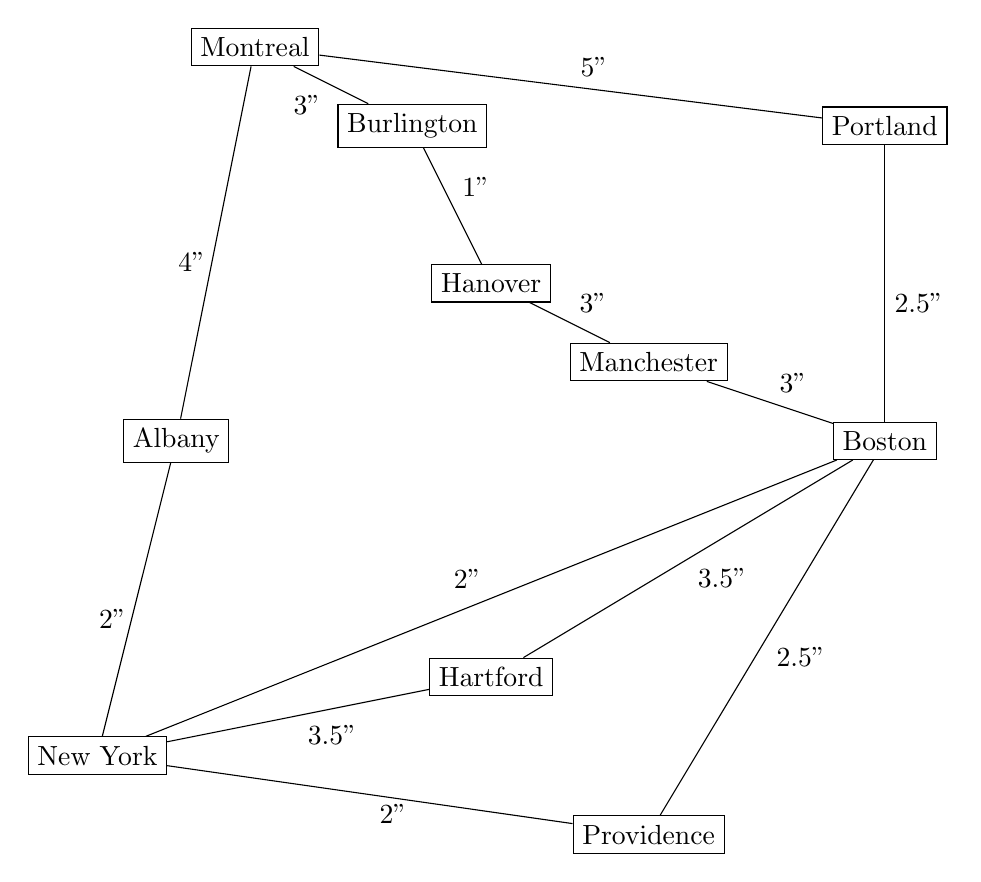
\begin{tikzpicture}
\node (New York) at (-2,0) [shape = rectangle, draw] {New York};

\node (Hartford) at (3, 1) [shape = rectangle, draw] {Hartford};

\node (Providence) at (5, -1) [shape=rectangle, draw] {Providence};

\node (Albany) at (-1,4) [shape=rectangle, draw] {Albany};

\node (Boston) at (8,4) [shape = rectangle, draw] {Boston};

\node (Manchester) at (5,5) [shape=rectangle, draw] {Manchester};

\node (Hanover) at (3, 6) [shape=rectangle, draw] {Hanover};

\node (Burlington) at (2, 8) [shape=rectangle, draw] {Burlington};

\node (Montreal) at (0,9) [shape=rectangle, draw] {Montreal};

\node (Portland) at (8,8) [shape=rectangle, draw] {Portland};


\path [-]   (New York)  edge  node[below left]  {2''}  (Albany)
    edge  node[above left]  {2''}  (Boston)
    edge  node[below right]  {3.5''}  (Hartford)
    edge  node[below right]  {2''}  (Providence)

  (Boston)  edge  node[below right]  {2.5''}  (Portland)
    edge  node[above right]  {3''}  (Manchester)
    edge  node[below right]  {3.5''}  (Hartford)
    edge  node[below right]  {2.5''}  (Providence)

  (Montreal)  edge  node[below left]  {3''}  (Burlington)
    edge  node[below left]  {4''}  (Albany)
    edge  node[above right]  {5''}  (Portland)
  
  (Hanover)  edge  node[above right]  {1''}  (Burlington)
    edge  node[above right]  {3''}  (Manchester);
\end{tikzpicture}

\subproblem Ignoring the labels, what is the edge connectivity of the region? What is the vertex connectivity?

\subproblem Now following the snowfall criterion for edge removal, what is the maximum amount of snowfall that would leave the region connected?

\subproblem Does the graph have any articulation points? Does it have any bridges? How would your answers change if 2 inches of snow fell on the region? Identify the articulation points or bridges if appropriate.

\begin{solution}

  \subsolution The edge connectivity is 2. The vertex connectivity is 2.

  \subsolution The maximum amount of snowfall that would leave the region connected is 2.5 inches.

  \subsolution The graph does not have any articulation points or bridges. If 2 inches of snow fell, Montreal and Manchester would become articulation points and Montreal-Burlington and Burlington-Hanover would become bridges.

\end{solution}

%% PROBLEM 2 %%
\problem{4}{6 lines}
Prove that if an edge is not part of any cycle, then it is a bridge.

\begin{solution}

Suppose an edge $e$ with endpoints $(u,v)$ is not part of any cycle. Since $u$ and $v$ are connected (by $e$), then they are in the same connected component. $e$ is the only path from $u$ to $v$ because if there were any other path $u, x_1, x_2, ... x_i, v$, then there would be a cycle $u, x_1, x_2, ... x_i, v, u$ using $e$. Therefore, if we remove $e$ from the graph, there is no path from $u$ to $v$. This means that $u$ and $v$ are in different connected components. Since $u$ and $v$ were originally in the same connected component, $e$ must be a bridge.

\end{solution}

\end{document}
